\documentclass[11pt]{article} 
\usepackage{amssymb, amsmath, amsthm}
\usepackage{tikz, graphicx, color, mathrsfs, rotating}
\usepackage{titlesec, lipsum}
\usepackage{fancyhdr, framed, chngcntr}

\usetikzlibrary{arrows,shapes,automata,backgrounds,decorations,petri,positioning,patterns}


\paperwidth = 8.5in
\paperheight = 11in
\textwidth = 6.5 in
\textheight = 9 in
\oddsidemargin = 0 in
\evensidemargin = 0 in
\topmargin = -.25 in
\headheight = 0.0 in
\headsep = .25 in
\footskip = .25in


\newtheorem*{repp@prob}{\repp@title}
\newcommand{\newreppprob}[2]{
\newenvironment{repp#1}[1]{
 \def\repp@title{#2 {##1}}
 \begin{repp@prob}}
 {\end{repp@prob}}}
\makeatother
\newreppprob{prob}{Problem}

\newtheorem*{repp@thm}{\repp@title}
\newcommand{\newreppthm}[2]{
\newenvironment{repp#1}[1]{
 \def\repp@title{#2 {##1}}
 \begin{repp@thm}}
 {\end{repp@thm}}}
\makeatother
\newreppthm{thm}{Theorem}


% -----------------------------------------------------------------------------
%             Macros for the course
% -----------------------------------------------------------------------------
\newcommand{\TS}{\mathcal{T}} % symbol for a topological space
\newcommand{\BS}{\mathcal{B}} % symbol for a basis
\newcommand{\R}{\mathbb{R}} % symbol for real numbers
\newcommand{\Z}{\mathbb{Z}} % symbol for integers
\newcommand{\Q}{\mathbb{Q}} % symbol for rational numbers
\newcommand{\PS}{\mathscr{P}} % symbol for power set
\newcommand{\E}{\mathbf{E}} % symbol for real numbers with Euclidean topology
\newcommand{\F}{\mathbf{F}^1} % symbol for real numbers with finite-complement topology
\renewcommand{\H}{\mathbf{H}^1} % symbol for real numbers with half-open topology
\renewcommand{\S}{\mathcal{S}} % basis topology
\newcommand{\B}{\mathbf{B}} % symbol for ball
\newcommand{\Sp}{\mathbf{S}} % symbol for sphere
\renewcommand{\int}{\operatorname{int}} % symbol for interior
\newcommand{\bnd}{\partial} % symbol for boundary
\newcommand{\homeo}{\approx} % symbol for homeomorphic


\begin{document} 


% -----------------------------------------------------------------------------
%             Start here
% -----------------------------------------------------------------------------

{\large
\noindent School of Computing %% replace "date" by the date on which the assignment was made
\hfill Chansu Park %% replace "Name" by your name

\vspace{.1in}

\noindent \today \hfill 20173245}

\vspace{.25in}

% -----------------------------------------------------------------------------
%             Erase or rearrange the options below, as necessary
% -----------------------------------------------------------------------------
\Large{
\begin{center}
\textbf{CS580}

Spring 2018, Homework \#2
\end{center}
}

\large

% -----------------------------------------------------------------------------
%             Template for typing up an Exercise
% -----------------------------------------------------------------------------
Here is the sample image only with point lights and a spotlight:
\begin{figure}[htb]
	\begin{center}
		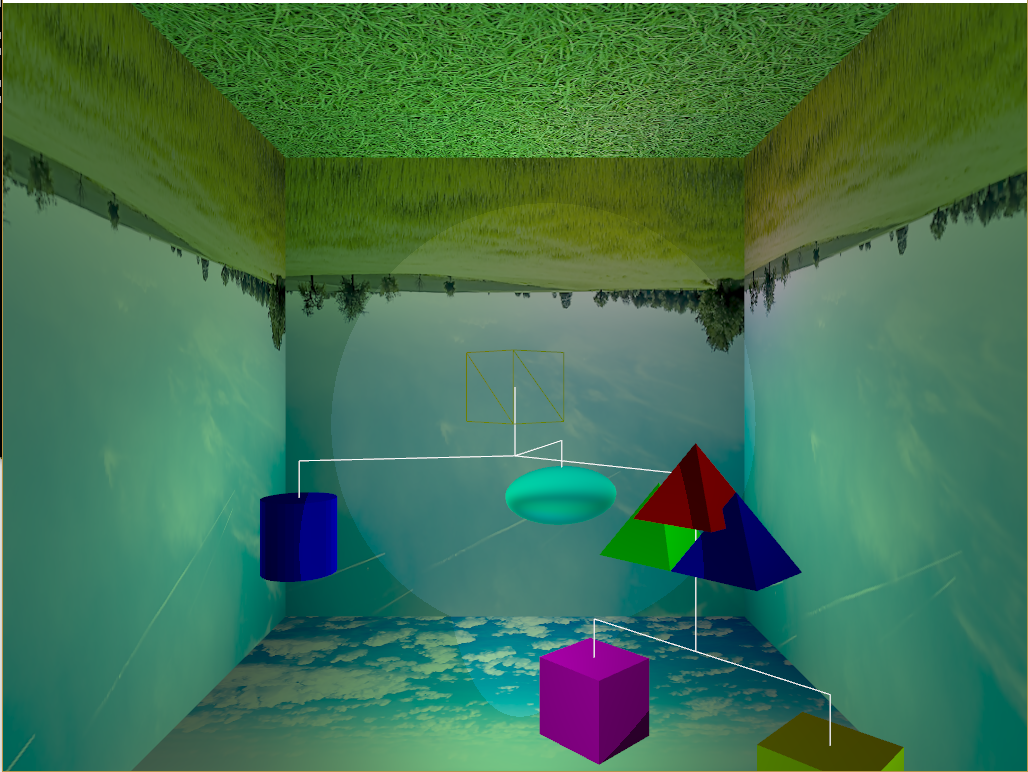
\includegraphics[width=0.8\linewidth]{pointSpot.png}
	\end{center}
	\caption{A sample picture with point lights and a spotlight. Note that there is also an ambient light.}
\end{figure}

\section{Lighting} \label{sec:1}
There are three components of the local lighting: ambient, diffuse, and specular.
Ambient light exists as a constant factor; diffuse/specular light depends on each material.

To simplify, I fixed diffuse factor $K_d$ as $0.4$; specular factor $K_s$ as $0.6$.
\newpage
\subsection{vertex shader} \label{ssec:1.1}
\begin{figure}[htb]
	\begin{center}
		\includegraphics[width=0.8\linewidth]{vertexshader.png}
	\end{center}
	\caption{Vertex shader. (VertexShader.glsl / TextureVertexShader.glsl)}
\end{figure}
The main problem on the original vertex shader (from the tutorial 2 of the CS580) was that the position of the fragment is clipped and then move on to the fragment shader.
Since the projection to the clip space from the view is not an affine transformation, it makes the light curved on the clip space.

Thus we have to take care the light before we clip the space to the canonical view volume, so I worked on the world coordinate for lighting.
Multiplying by model transform and multipliying by the inverse of the model transformation move each position and normal vector from the model to the space, respectively.
Then the vertex shader gives these two information to the fragment shader.

Note that, for the texture, the last line will be changed to \texttt{fragmentUV=vertex\_uv;}.

\subsection{fragment shader} \label{ssec:1.2}
Fragment shader takes five information from the vertex shader: fragment color (fragment parameter for the texture), fragment position(clip space / world space), and fragment normal(clip space / world space).

It also takes several uniform variables:
\begin{itemize}
	\item [directional lights:] light vector (already inversed), color
	\item [point lights:] position of the light point, color, attenuation terms
	\item [spot light:] variables that the point light takes + center direction of the light, angle of the cone of the spot light
	\item [transformations:] Model to world (ModelTransform), world to view (Eye), projection (Projection)
	\item [light switches:] \texttt{light[6]}: Turn on/off each lights
	\item [alpha:] surface smoothness
	\item [diffuse, specular:] \texttt{d, s}: constants for diffuse/specular term
	\item [blinn:] switches between Phong model and Blinn-Phong model.
\end{itemize}
There are three functions for each lights: \texttt{directionalLight, pointLight, spotLight} which take fragment normal vector and view vector from the fragment to the camera in common: each according to the world coordinate, and an instance of each light type.
\subsubsection{directional light} \label{sssec:1.2.1}
\begin{figure}[htb]
	\begin{center}
		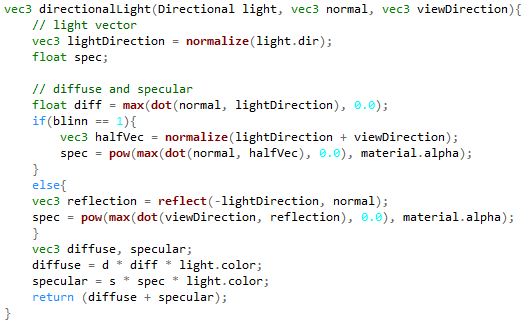
\includegraphics[width=0.7\linewidth]{directional.png}
	\end{center}
	\caption{Code for the directionalLight function.}
\end{figure}
Compute the normalized light vector; compute diffuse and specular intensity according to Blinn-Phong or Phong model; then add them with diffuse/specular coefficient. No attenuation term is needed since it is directional light.
\newpage
\subsubsection{point light} \label{sssec:1.2.2}
\begin{figure}[htb]
	\begin{center}
		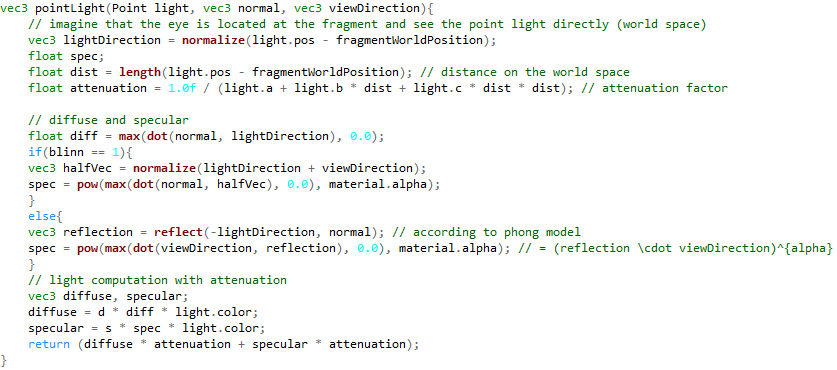
\includegraphics[width=1.0\linewidth]{point.png}
	\end{center}
	\caption{Code for the pointLight function.}
\end{figure}
Compute the normalized light vector; compute diffuse and specular intensity according to Blinn-Phong or Phong model; then add them with diffuse/specular coefficient and the attenuation term.
\subsubsection{spot light} \label{sssec:1.2.3}
It is almost the same as the point light, but the caller \texttt{main()} restricts the computation with the angle between the center direction of the light and the view vector.

\begin{figure}[htb]
	\begin{center}
		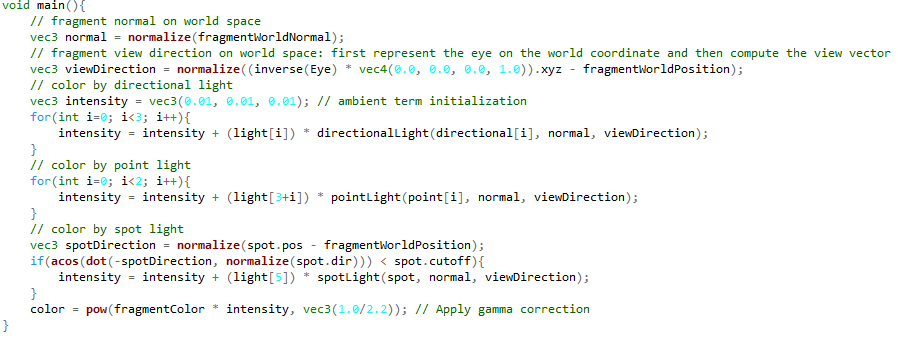
\includegraphics[width=1.0\linewidth]{main.png}
	\end{center}
	\caption{Main function of the fragment shader (FragmentShader/TextureFragmentShader.glsl).}
\end{figure}

The main function of the fragment shader first initialize the light with the ambient term and then add lights, and finally apply the gamma correction on the product of the fragment color (texture color for the texture fragment shader) and the intensity.

Note that, I didn't use \texttt{light.cpp/light.hpp}. Instead, I gave the information for each fragment on the \texttt{textureModel/colorModel.cpp}. You can see that in the \texttt{Draw()} function. Here are the information for each light source (each points / vectors are on the world coordinate):
\begin{itemize}
	\item[directional lights:] Light vector: (1,1,1) with color Red/Blue/Green
	\item[point lights:] attenuation: 1 for constant; 0.1 for the linear term; 0.1 for the quadratic term.
	\begin{itemize}
		\item [(i)] Light position: (2, 3, -2) / Color: (0.8, 0, 0.8).
		\item [(ii)] Light Position: (0, -3, 3) / Color: (0.25, 0.75, 0.25).
	\end{itemize}
	\item[spot light:] attenuation: (1, 0, 0.01), Light Position: (-1, -4, 10), Light direction (central vector of the spotlight): (0.1, 0.2, -1), cone angle: \texttt{atan(0.3)}.
\end{itemize}

I also mapped keys: B-button for the switch between Blinn-Phong/Phong Model, 1~6 buttons for switching lights.

\section{Texture Mapping for wall and floor} \label{sec:2}
Setting texture is similar to create texture for Render-to-Texture mapping introduced in the tutorial 2. Thus I implemented \texttt{SetTexture(const char *name)} which takes the relative location and then attach that image at the location as a texture to the surface.
\begin{figure}[htb]
	\begin{center}
		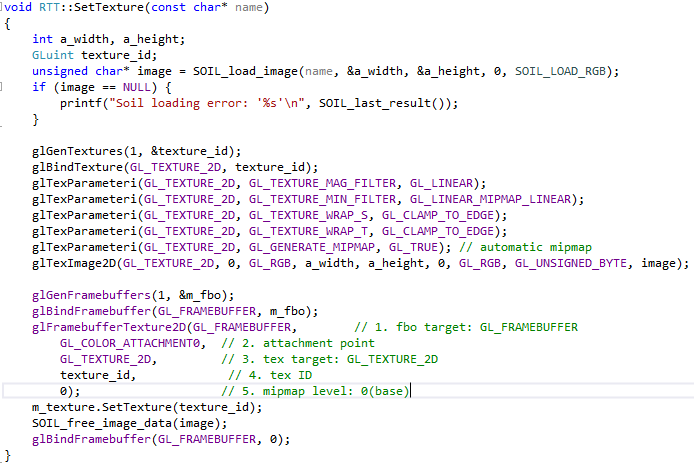
\includegraphics[width=0.7\linewidth]{rttSetTexture.png}
	\end{center}
	\caption{Similar to the \texttt{CreateTexture} method, but it uses SOIL library.}
\end{figure}
First, it reads the image as an unsigned byte array using SOIL library, and then attach it with a certain \texttt{texture\_id}.
\newpage
\begin{figure}[htb]
	\begin{center}
		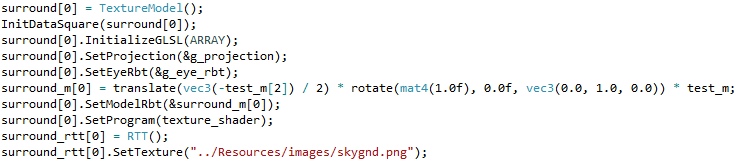
\includegraphics[width=1.0\linewidth]{mainSurround.png}
	\end{center}
	\caption{Generate \texttt{TextureModel} instance for the geometry, and make an \texttt{RTT} instance.}
\end{figure}
\begin{figure}[htb]
	\begin{center}
		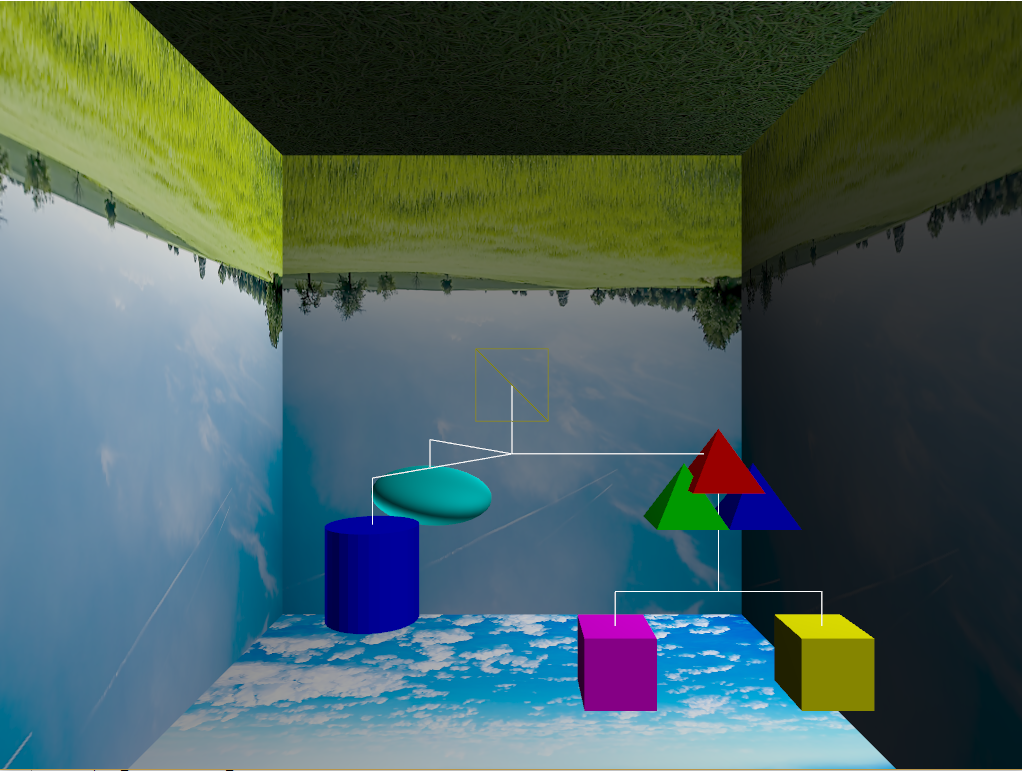
\includegraphics[width=0.8\linewidth]{directionalLight.png}
	\end{center}
	\caption{Since the normal vector for the ceiling and the right wall has more than 90 degree with the directional light, they wouln't be affected: compare with figure 1.}
\end{figure}

\section{Creativity} \label{sec:3}
The lighting method switching (Blinn-Phong / Phong) is the only one that I implemented more.
\newpage

\section{Directory hierarchy}
I worked on \texttt{Visual Studio 2015 Professional Win64}.

This time, I attached the whole sources from the skeleton zip file since I edited several files.

You can see the images I used for textures in the \texttt{./Resources/images/}.

For the executable, the \texttt{Executable} folder contains the copy of the executable from \texttt{./build/Debug} with shaders from \texttt{./Skeleton}.

There is also a pdf file containing this document in the root. Hope you to see this program.

%\begin{proof}[Solution.]
%% write your solution here
%\end{proof}


% -----------------------------------------------------------------------------
%             Template for typing up a Theorem
% -----------------------------------------------------------------------------
%\begin{reppthm}{42} %% replace "42" by the relevant Theorem number
%% restate the Theorem here
%\end{reppthm}

%\begin{proof}
%% write your proof here
%\end{proof}


% -----------------------------------------------------------------------------
%             End here
% -----------------------------------------------------------------------------

\end{document}